\chapter{SCI-HI System Development}\label{Ch:System}

\section{Overview}
$''$Sonda Cosmologica de las Islas para la Deteccion de Hidrogeno Neutro$''$ (SCI-HI) is an experiment which seeks to measure the \cm global spectrum during the end of the Dark Ages and the Cosmic Dawn before reionization. As such, SCI-HI instrument was designed to meet several distinct contraints:

\begin{enumerate}
\item The design must be low cost (under \$ 10,000 \textcolor{red}{Is this the right range?}).

\item The design must be low power (under \textcolor{red}{What value should this be?}) and be able to run with an independent power source separate from external supplies. 

\item The design must be simple and easy to deploy to remote locations. 

\item The design must be broad-band to cover the wide bandwidth of interest ($30-140$ MHz).

\end{enumerate}

\begin{figure}[htb]
\begin{center}
\includegraphics[width=0.9\linewidth]{SCIHI_system/figures/basic_block_diagram.png}
\caption{Basic Block Diagram of the SCI-HI instrument.}
\label{Fig:basic_block_diagram}
\end{center}
\end{figure}

In order to meet these constraints, the instrument design was broken down into three categories based upon their purpose in the overall design (see Figure \ref{Fig:basic_block_diagram}). These categories are an antenna for signal collection, radio frequency (RF) electronics for signal transmission, and a computer for signal processing and storage.

\section{Antenna}
When designing an instrument for radio astronomy, one of the big challenges is finding an antenna design that fits the particular needs of a given experiment. 

\subsection{Design Considerations}
For the SCI-HI experiment, the key properties for the antenna selection were the bandwidth and stability of the antenna beam pattern and impedance (S-parameters) over frequency. 

\textcolor{red}{Here I will add a brief discussion of antenna design including some of the key parameters for an antenna in general and why they are significant. }

\begin{figure}[htb]
\centering
\begin{minipage}[b]{0.45\textwidth}
\centering
\includegraphics[width=0.95\linewidth]{SCIHI_system/figures/trombone_guad_small.jpg}
\caption{Trombone Antenna setup in its smallest (highest center frequency) configuration.}
\label{Fig:trombone_small}
\end{minipage}%
\begin{minipage}[b]{0.02\textwidth}
\hspace{1cm}
\end{minipage}%
\begin{minipage}[b]{0.51\textwidth}
\centering
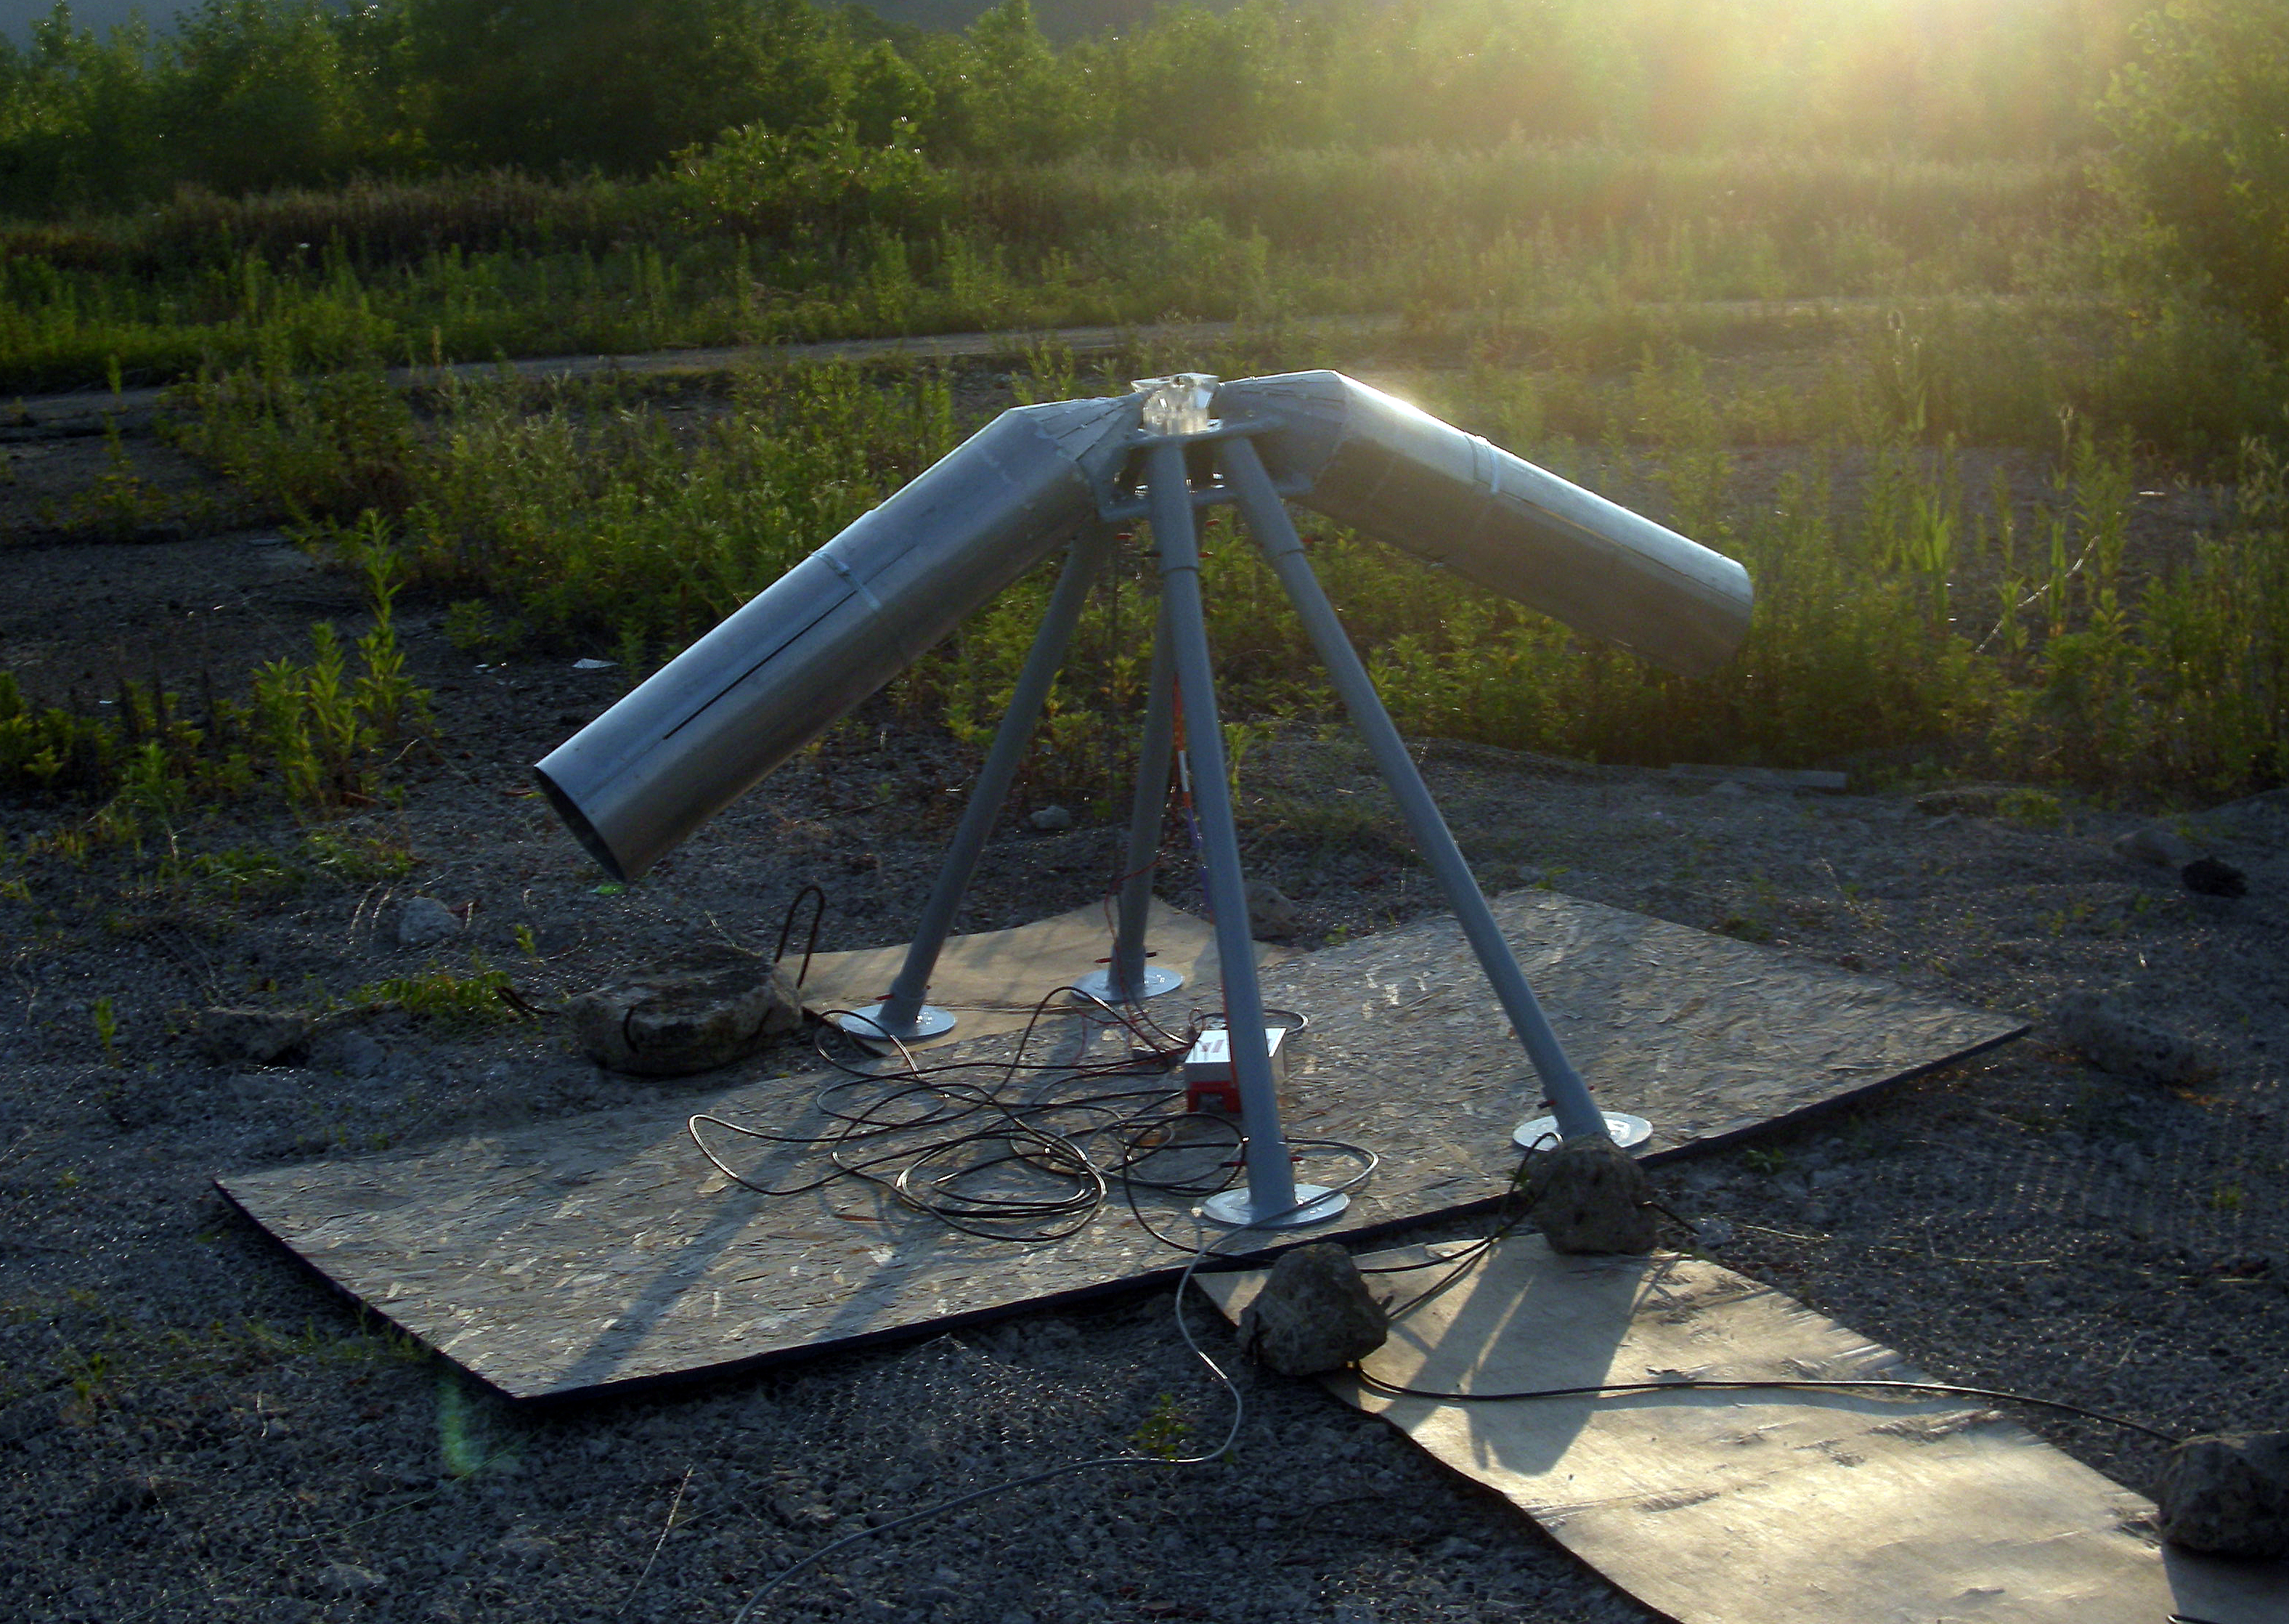
\includegraphics[width=0.95\linewidth]{SCIHI_system/figures/trombone_pgh_zoom.jpg}
\caption{Trombone Antenna setup in its largest (lowest center frequency) configuration.}
\label{Fig:trombone_large}
\end{minipage}
\end{figure}

\subsection{First Stage Antenna}
Initially, we started with a simple $''$Trombone$''$ antenna. This design is a dipole with fat, angled elements over a ground plane (see Figures \ref{Fig:trombone_small} and \ref{Fig:trombone_large}). Changing the frequency range of the antenna simply required shifting the length of the dipole elements and their position above the ground plane. 

\begin{figure}[htb]
\centering
\begin{minipage}[b]{0.53\textwidth}
\centering
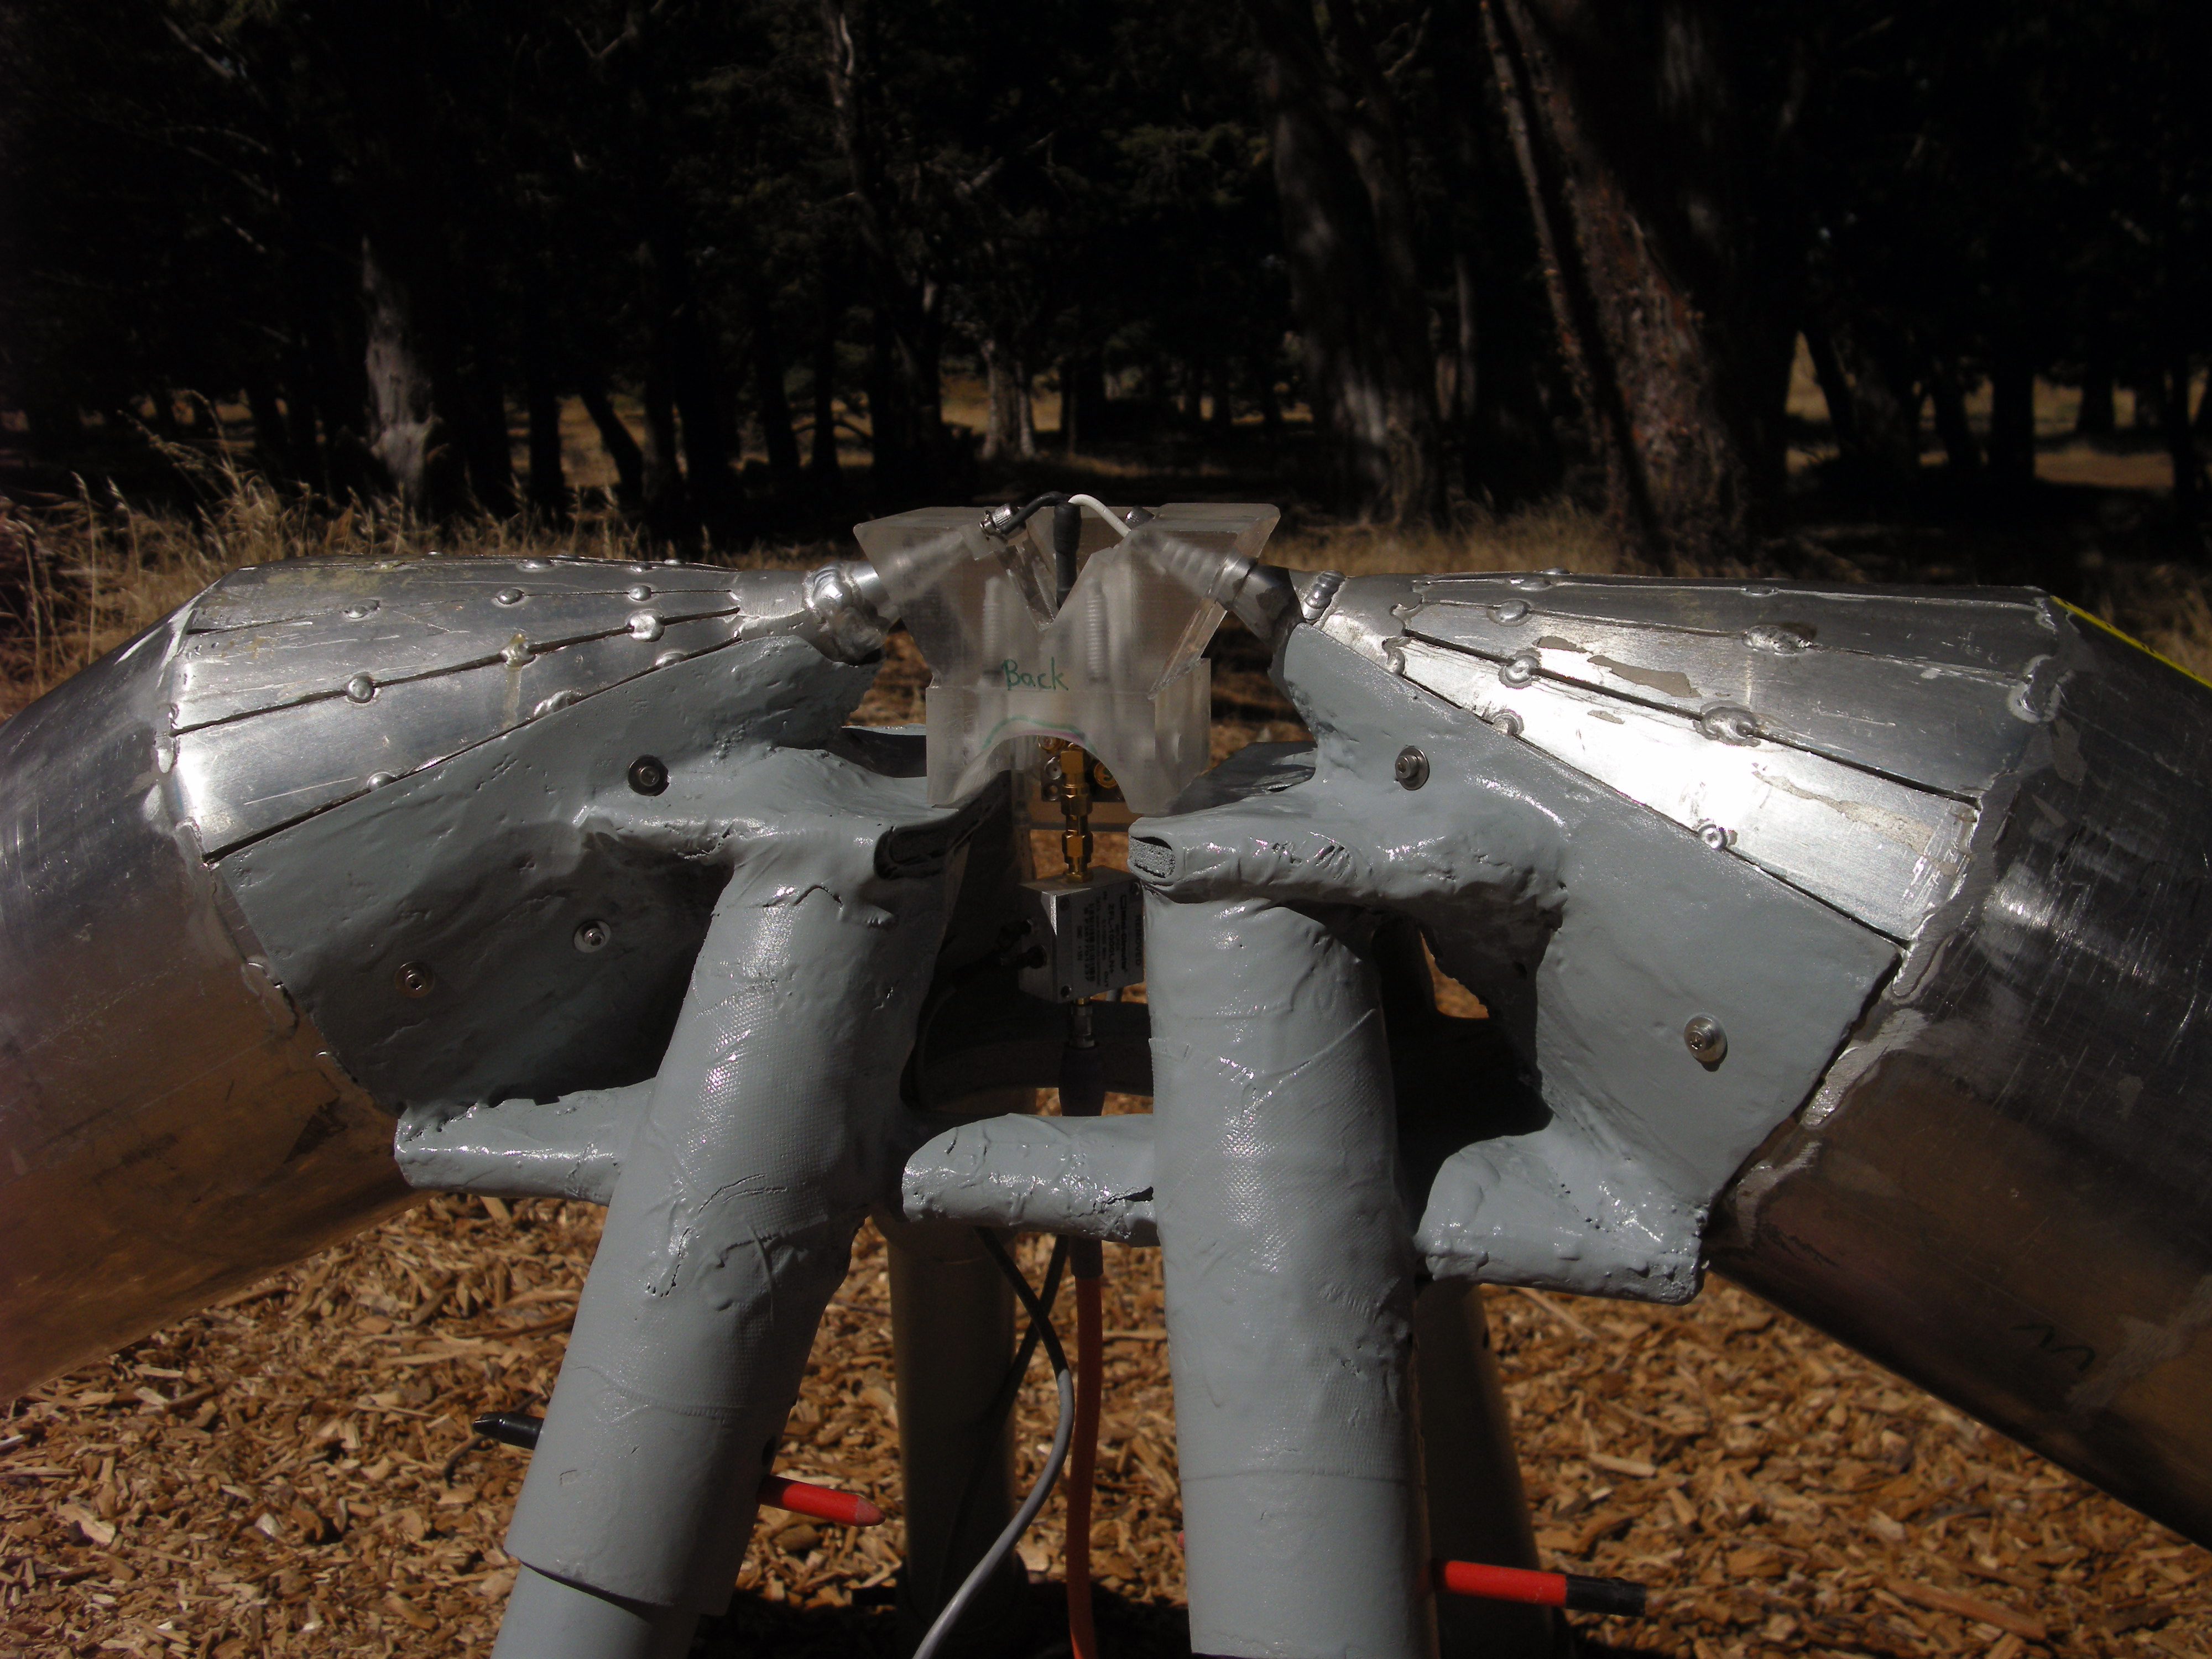
\includegraphics[width=0.95\linewidth]{SCIHI_system/figures/trombone_mount.jpg}
\caption{Mounting for the Trombone antenna, with lucite mount point and fiberglass support structure. }
\label{Fig:trombone_mount}
\end{minipage}%
\begin{minipage}[b]{0.02\textwidth}
\hspace{1cm}
\end{minipage}%
\begin{minipage}[b]{0.41\textwidth}
\centering
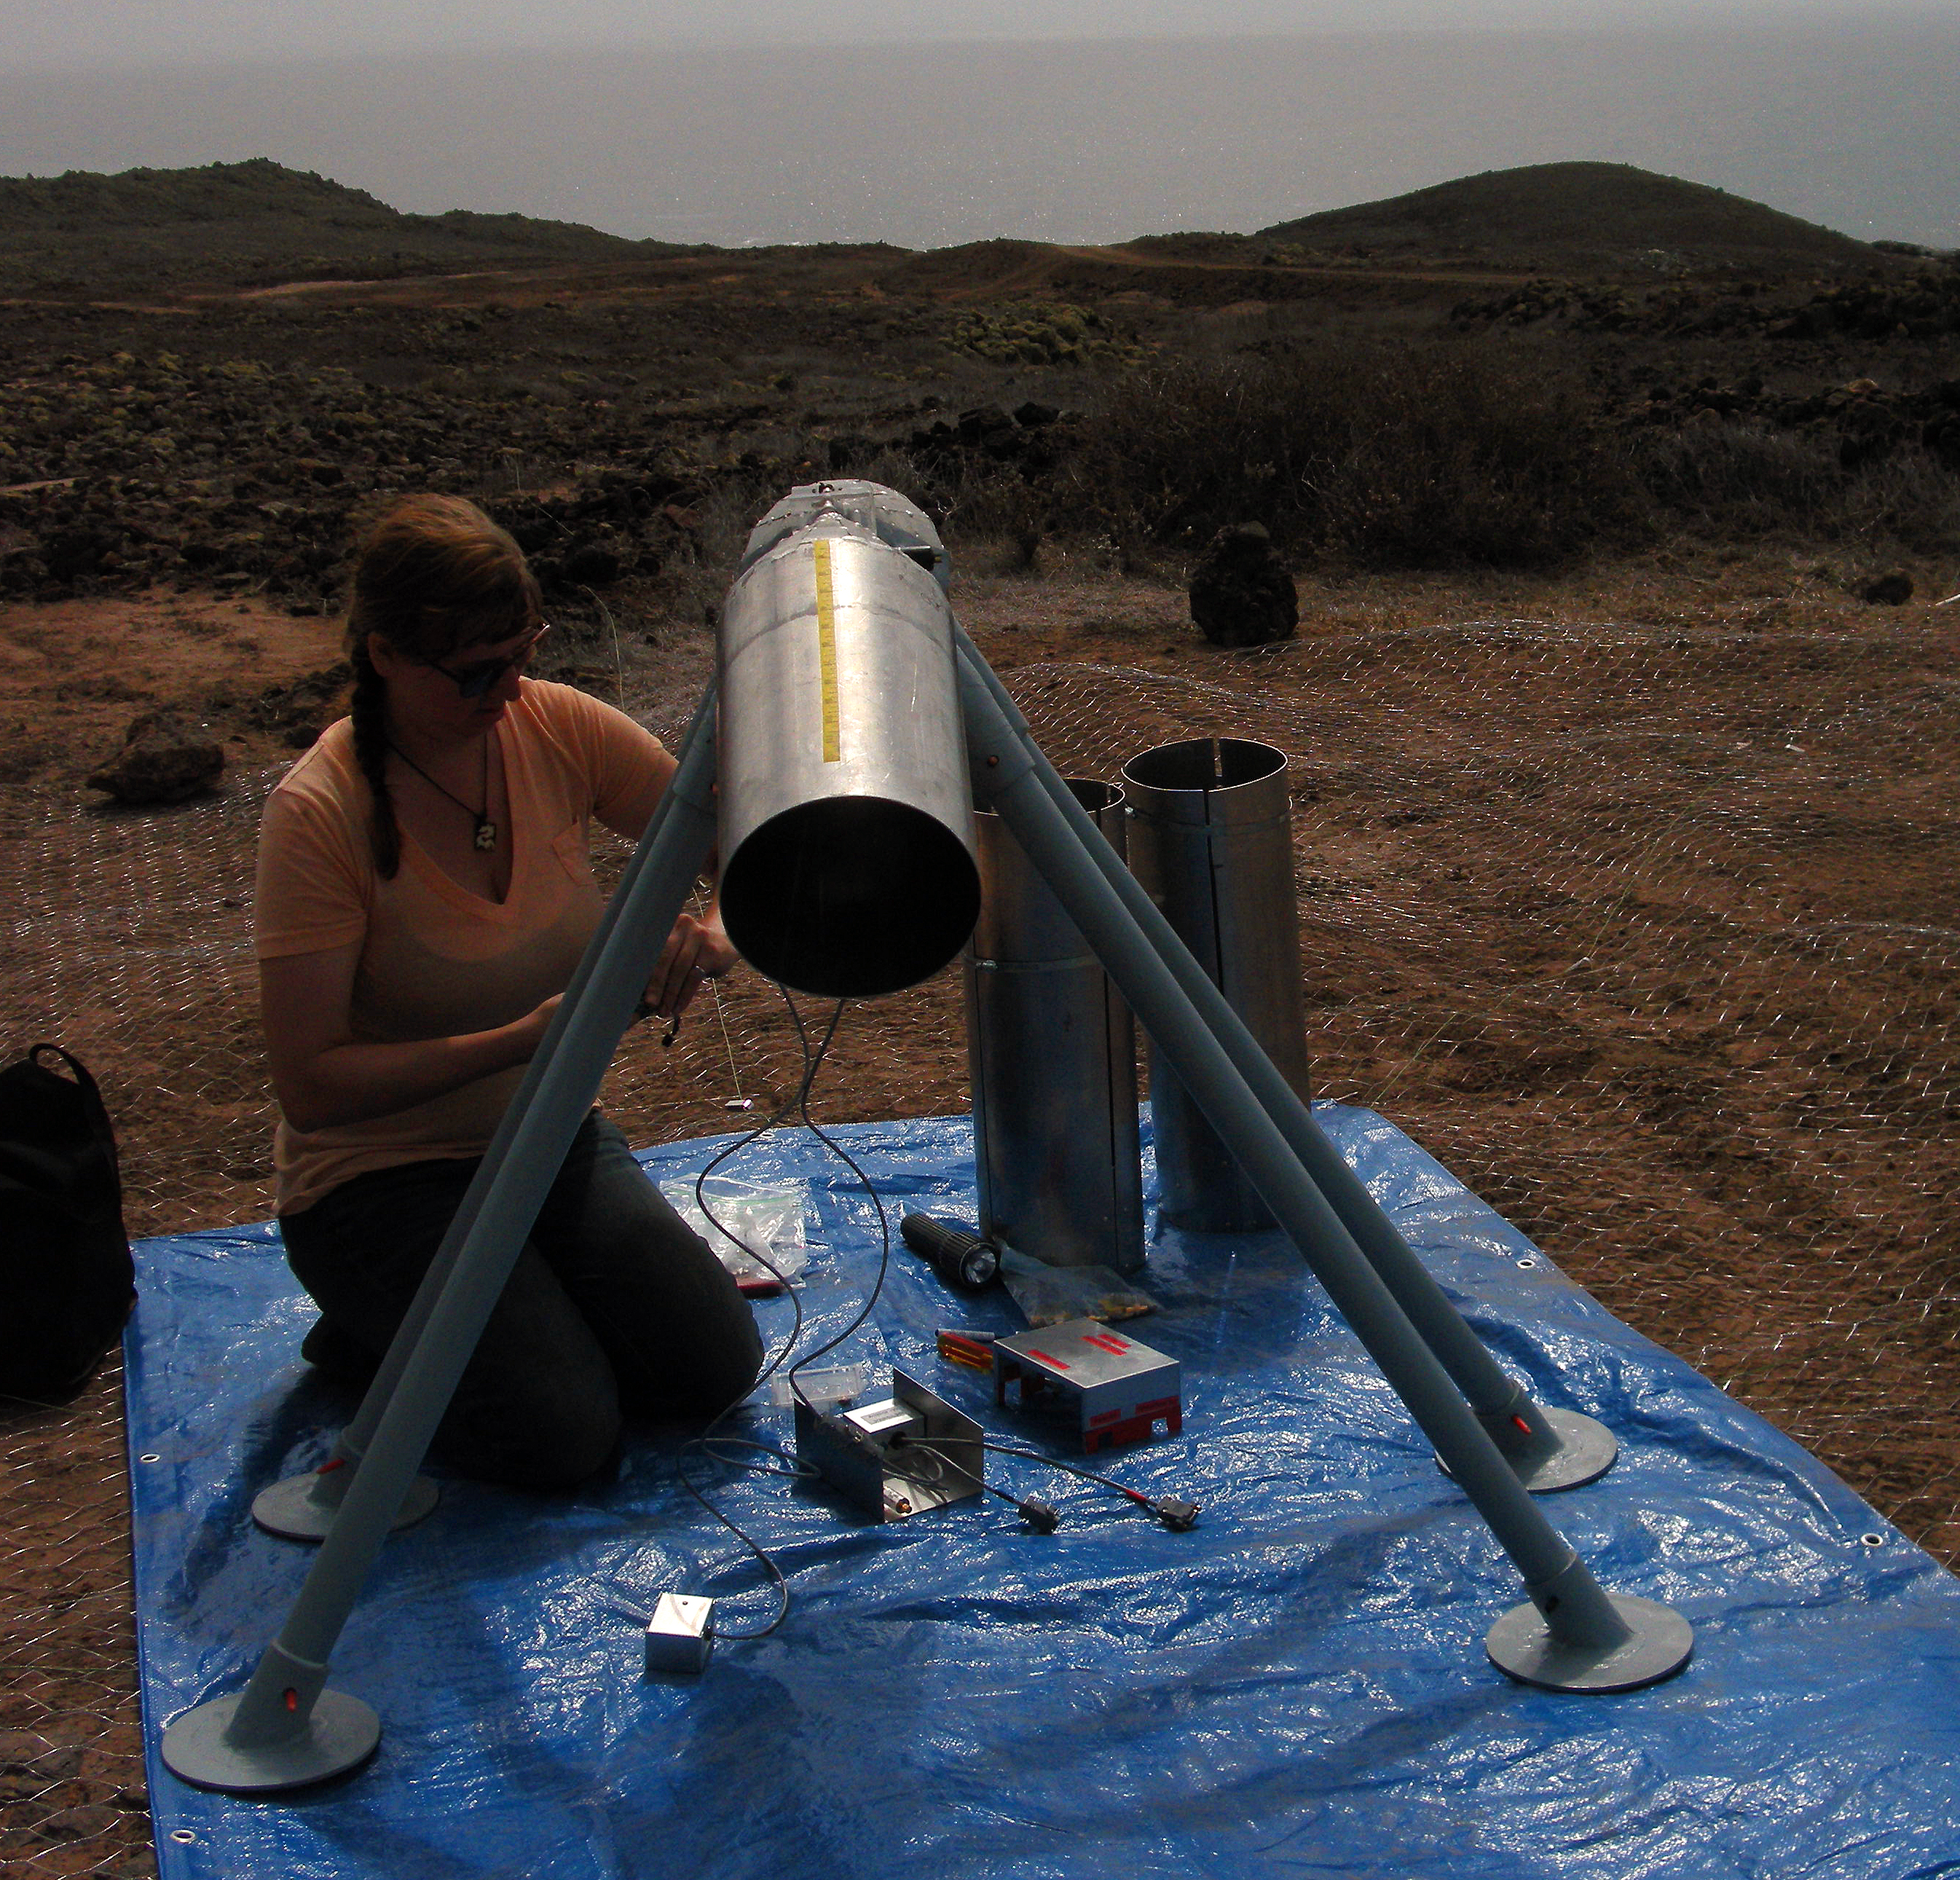
\includegraphics[width=0.95\linewidth]{SCIHI_system/figures/trombone_guad_adj.jpg}
\caption{Changing the Trombone antenna configuration from small to large.}
\label{Fig:trombone_adj}
\end{minipage}
\end{figure}

\subsubsection{Antenna Construction}
The trombone shapes were constructed out of welded aluminum with a lucite mounting block at the connection point of the two cones (see Figure \ref{Fig:trombone_mount}), The dipoles and mounting block were supported with a structure constructed out of fiberglass and PVC tubes. The entire system was placed above a ground plane composed of metal mesh (aka chicken wire) over a small ($\sim9 m^2$) area and long wire extensions ($\sim10 m$) extending out from the center like a spider web. 

Tuning the trombone length was accomplished with an external tube that slid over the main dipole elements (see Figure \ref{Fig:trombone_adj}), while adjusting the height of the trombone was done using the support legs (PVC pipes with variable heights).

The Trombone antenna was used throughout the initial stages of the SCI-HI project, including deployments at Green Bank in West Virginia (Figure \ref{Fig:trombone_gbt}), the Zona del Silencio in Mexico (Figure \ref{Fig:trombone_zds}), Algonquin Radio Observatory in Canada (Figure \ref{Fig:trombone_alg}), and Isla Guadalupe in Mexico (Figure \ref{Fig:trombone_guad}). For more discussion of these sites, see Chapter \ref{Ch:RFI_test}.

\begin{figure}[htb]
\centering
\begin{minipage}[b]{0.48\textwidth}
\centering
\includegraphics[width=0.95\linewidth]{SCIHI_system/figures/trombone_gbt.jpg}
\caption{SCI-HI setup with trombone antenna on site at Green Bank in August 2011.}
\label{Fig:trombone_gbt}
\end{minipage}%
\begin{minipage}[b]{0.02\textwidth}
\hspace{1cm}
\end{minipage}%
\begin{minipage}[b]{0.46\textwidth}
\centering
\includegraphics[width=0.95\linewidth]{SCIHI_system/figures/trombone_sys_ZdS.jpg}
\caption{SCI-HI setup with trombone antenna on site at the Zona del Silencio in January 2012.}
\label{Fig:trombone_zds}
\end{minipage}
\end{figure}

\begin{figure}[htb]
\centering
\begin{minipage}[b]{0.52\textwidth}
\centering
\includegraphics[width=0.95\linewidth]{SCIHI_system/figures/trombone_alg_sys.jpg}
\caption{SCI-HI setup with trombone antenna on site at the Algonquin Radio Observatory in August 2012.}
\label{Fig:trombone_alg}
\end{minipage}%
\begin{minipage}[b]{0.02\textwidth}
\hspace{1cm}
\end{minipage}%
\begin{minipage}[b]{0.42\textwidth}
\centering
\includegraphics[width=0.95\linewidth]{SCIHI_system/figures/trombone_sys_guad.jpg}
\caption{SCI-HI setup with trombone antenna on site at Isla Guadalupe in October 2012.}
\label{Fig:trombone_guad}
\end{minipage}
\end{figure}

\subsubsection{Antenna Simulation}
Simulating the Trombone antenna indicated some problems with the design, including significant structure in the antenna beam and S-parameters. \textcolor{red}{Add image/details of Amy's simulation results.}

\subsection{HIbiscus Antenna Design}

Because of the problems we had with the trombone design, we decided to shift our antenna design in a new direction based upon our expectations from the literature (\textcolor{red}{Need to add specific references for different antenna types}). We tested several antenna designs in simulation, including the four-square design used in the EDGES experiment \cite{rogers_2012}. This testing was done using FEKO, a finite element computational electromagnetics software package.\footnote{https://www.feko.info/}

Based on the FEKO simulation results we settled on a design that used the EDGES design as a starting point, but changed the exact shapes of the four squares. We took each square and turned it into an incliclined petal composed of three trapezoidal shapes. Each shape was connected to its neighbors on the petal, but had a different angle with respect to the ground. Additional panels were added to each side of the petal to create a strip line with a fixed gap between the petals. The entire antenna was then placed a distance above a flat ground plane. We call this design a HIbiscus antenna. 

\textcolor{red}{Add either pictures or simulation images for antenna shape details.}

We found that the shape parameters that were most significant in affecting antenna performance were the strip line gap width and the height of the antenna with respect to the ground plane. 


\begin{figure}[htb]
\centering
\begin{minipage}[b]{0.51\textwidth}
\centering
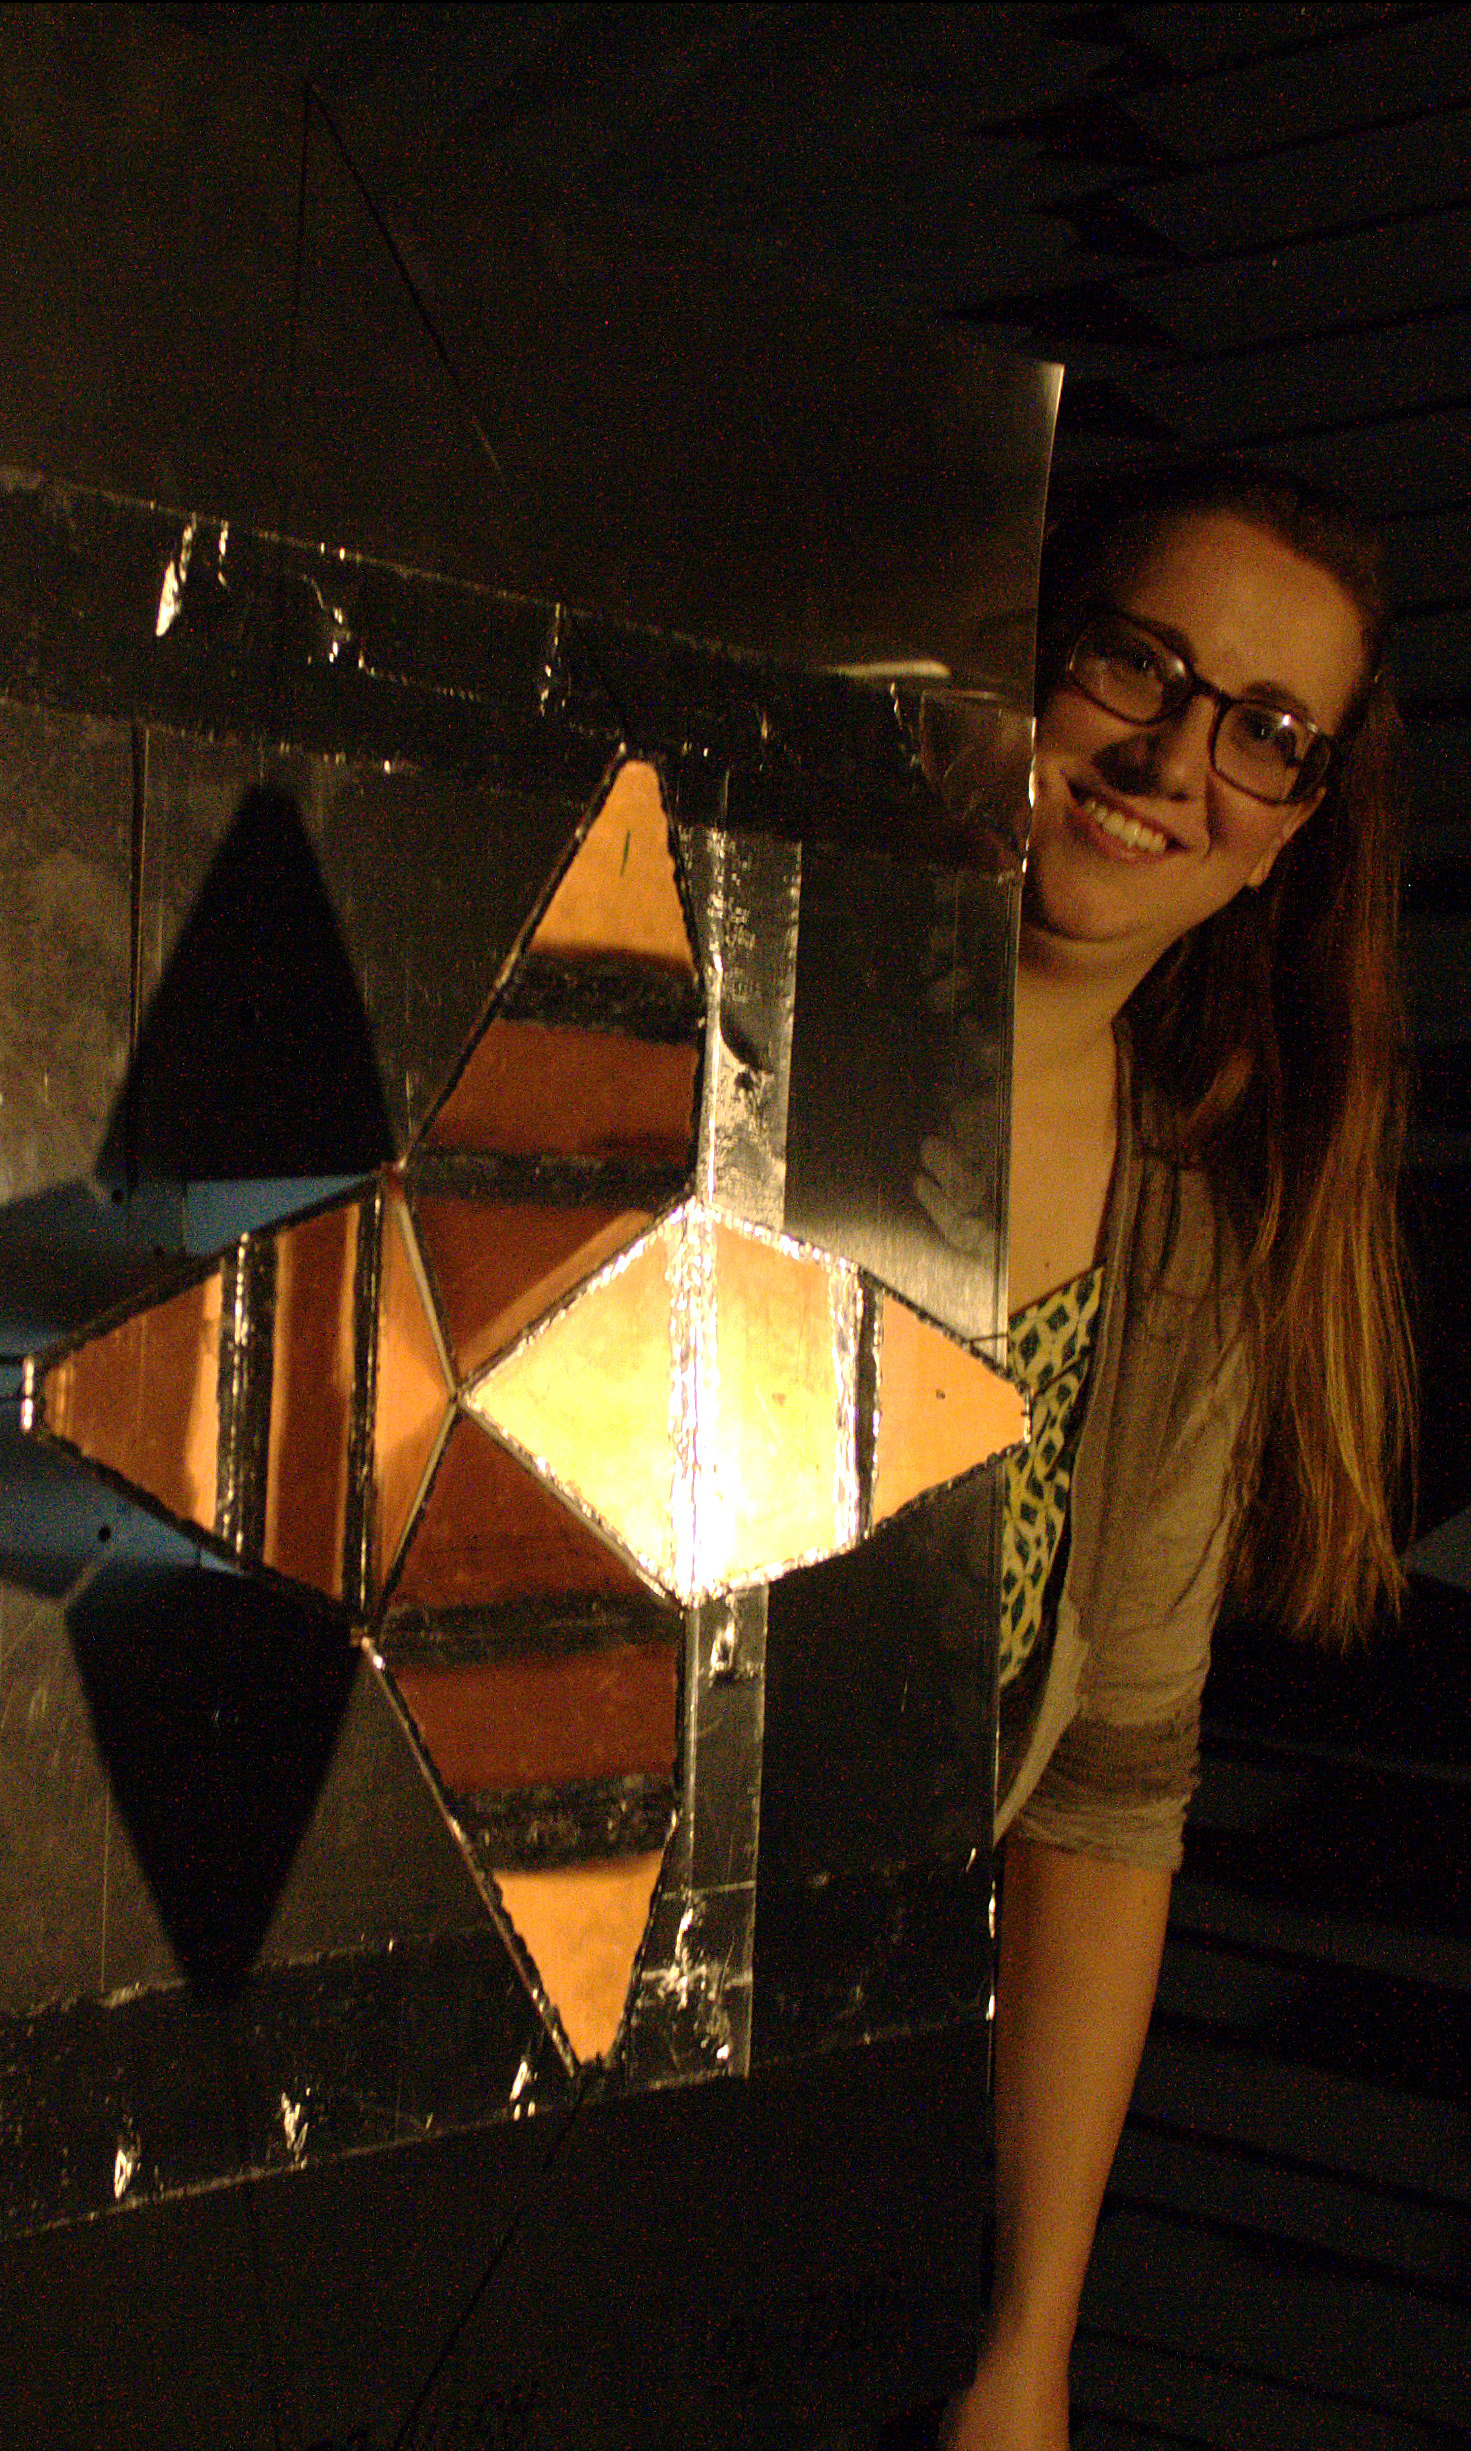
\includegraphics[width=0.95\linewidth]{SCIHI_system/figures/model_test_tabitha.jpg}
\caption{Testing a model HIbiscus antenna in the Project REAL Chamber. }
\label{Fig:hibiscus_scale_tabitha}
\end{minipage}%
\begin{minipage}[b]{0.02\textwidth}
\hspace{1cm}
\end{minipage}%
\begin{minipage}[b]{0.43\textwidth}
\centering
\includegraphics[width=0.95\linewidth]{SCIHI_system/figures/model_test_jose.jpg}
\caption{Scale model test with a different HIbiscus antenna model.}
\label{Fig:hibiscus_scale_jose}
\end{minipage}
\end{figure}

\subsubsection{Scale Model Testing}
In order to test our simulation to see if it matched the real antenna performance, we built a set of scaled HIbiscus designs tuned for higher frequencies around 400 MHz. This allowed us to use an antenna range to measure the antenna beam shape and s-parameters. 

We used the Project REAL\footnote{http://www.preal.ece.cmu.edu/} (Remote Educational Antenna Laboratory) facility at Carnegie Mellon University to measure the antenna response of different scaled HIbiscus models, as is shown in Figures \ref{Fig:hibiscus_scale_tabitha} and \ref{Fig:hibiscus_scale_jose}. By incrementally adjusting the strip line gap width and antenna height we were able to tune the antenna scale model to optimize these critical parameters in a real design. 

Using the scale model data, we were also able to edit the antenna simulation to better match the actual antenna response, providing us with an antenna simulation dataset that was closer to reality. 

\textcolor{red}{Here there will be some paragraphs about the exact simulation and scale model measurements including plots of impedence and antenna pattern.}

\begin{figure}[htb]
\centering
\begin{minipage}[b]{0.43\textwidth}
\centering
\includegraphics[width=0.95\linewidth]{SCIHI_system/figures/HIbiscus_pgh_imp.jpg}
\caption{HIbiscus antenna scaled for 70 MHz as it was setup during s-parameter testing at CMU. }
\label{Fig:hibiscus_first}
\end{minipage}%
\begin{minipage}[b]{0.02\textwidth}
\hspace{1cm}
\end{minipage}%
\begin{minipage}[b]{0.51\textwidth}
\centering
\includegraphics[width=0.95\linewidth]{SCIHI_system/figures/HIbiscus_gbt.jpg}
\caption{HIbiscus antenna scaled for 70 MHz setup for s-parameter testing on site at Green Bank.}
\label{Fig:hibiscus_gbt}
\end{minipage}
\end{figure}

\subsection{HIbiscus Antenna Construction}

\subsubsection{Initial Assembly}
Once we had a design finalized, we set out to construct a HIbiscus antenna with its center frequency tuned to 70 MHz (in the middle of the SCI-HI observation band).

\begin{figure}[htb]
\centering
\begin{minipage}[b]{0.40\textwidth}
\centering
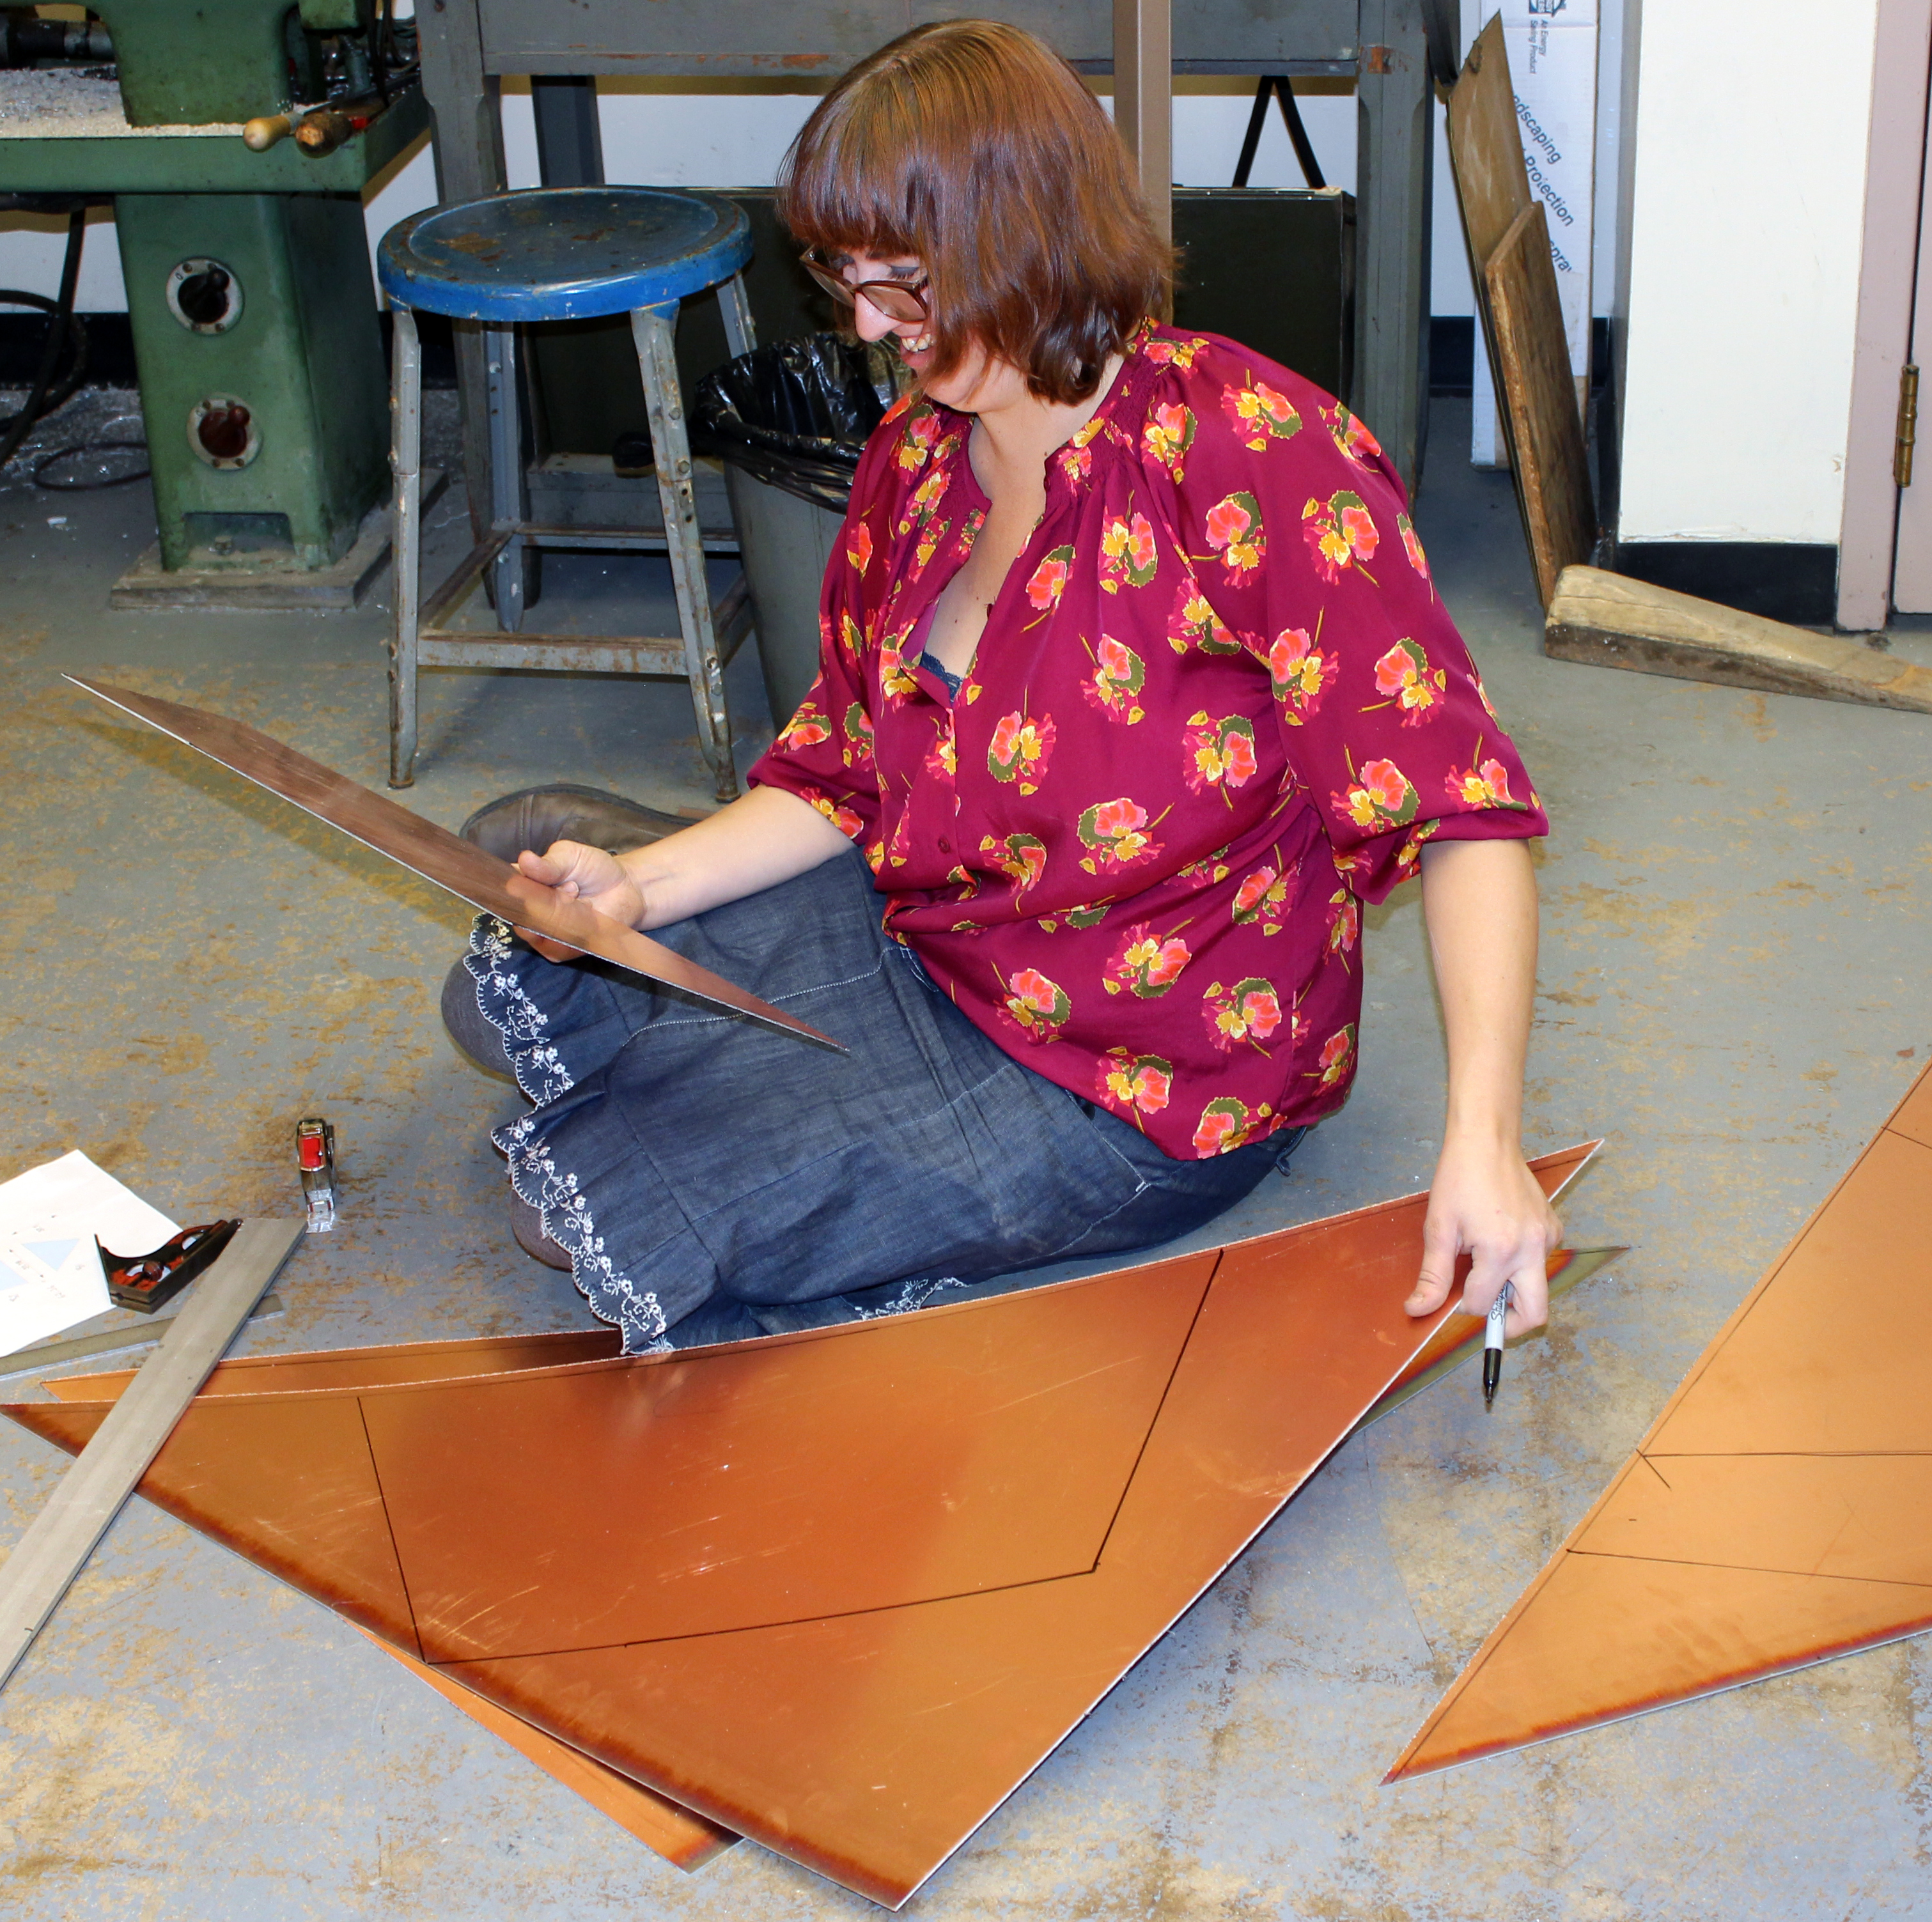
\includegraphics[width=0.95\linewidth]{SCIHI_system/figures/HIbiscus_pcb_cut.jpg}
\caption{HIbiscus antenna pcb panels being cut. }
\label{Fig:hibiscus_pcb}
\end{minipage}%
\begin{minipage}[b]{0.02\textwidth}
\hspace{1cm}
\end{minipage}%
\begin{minipage}[b]{0.54\textwidth}
\centering
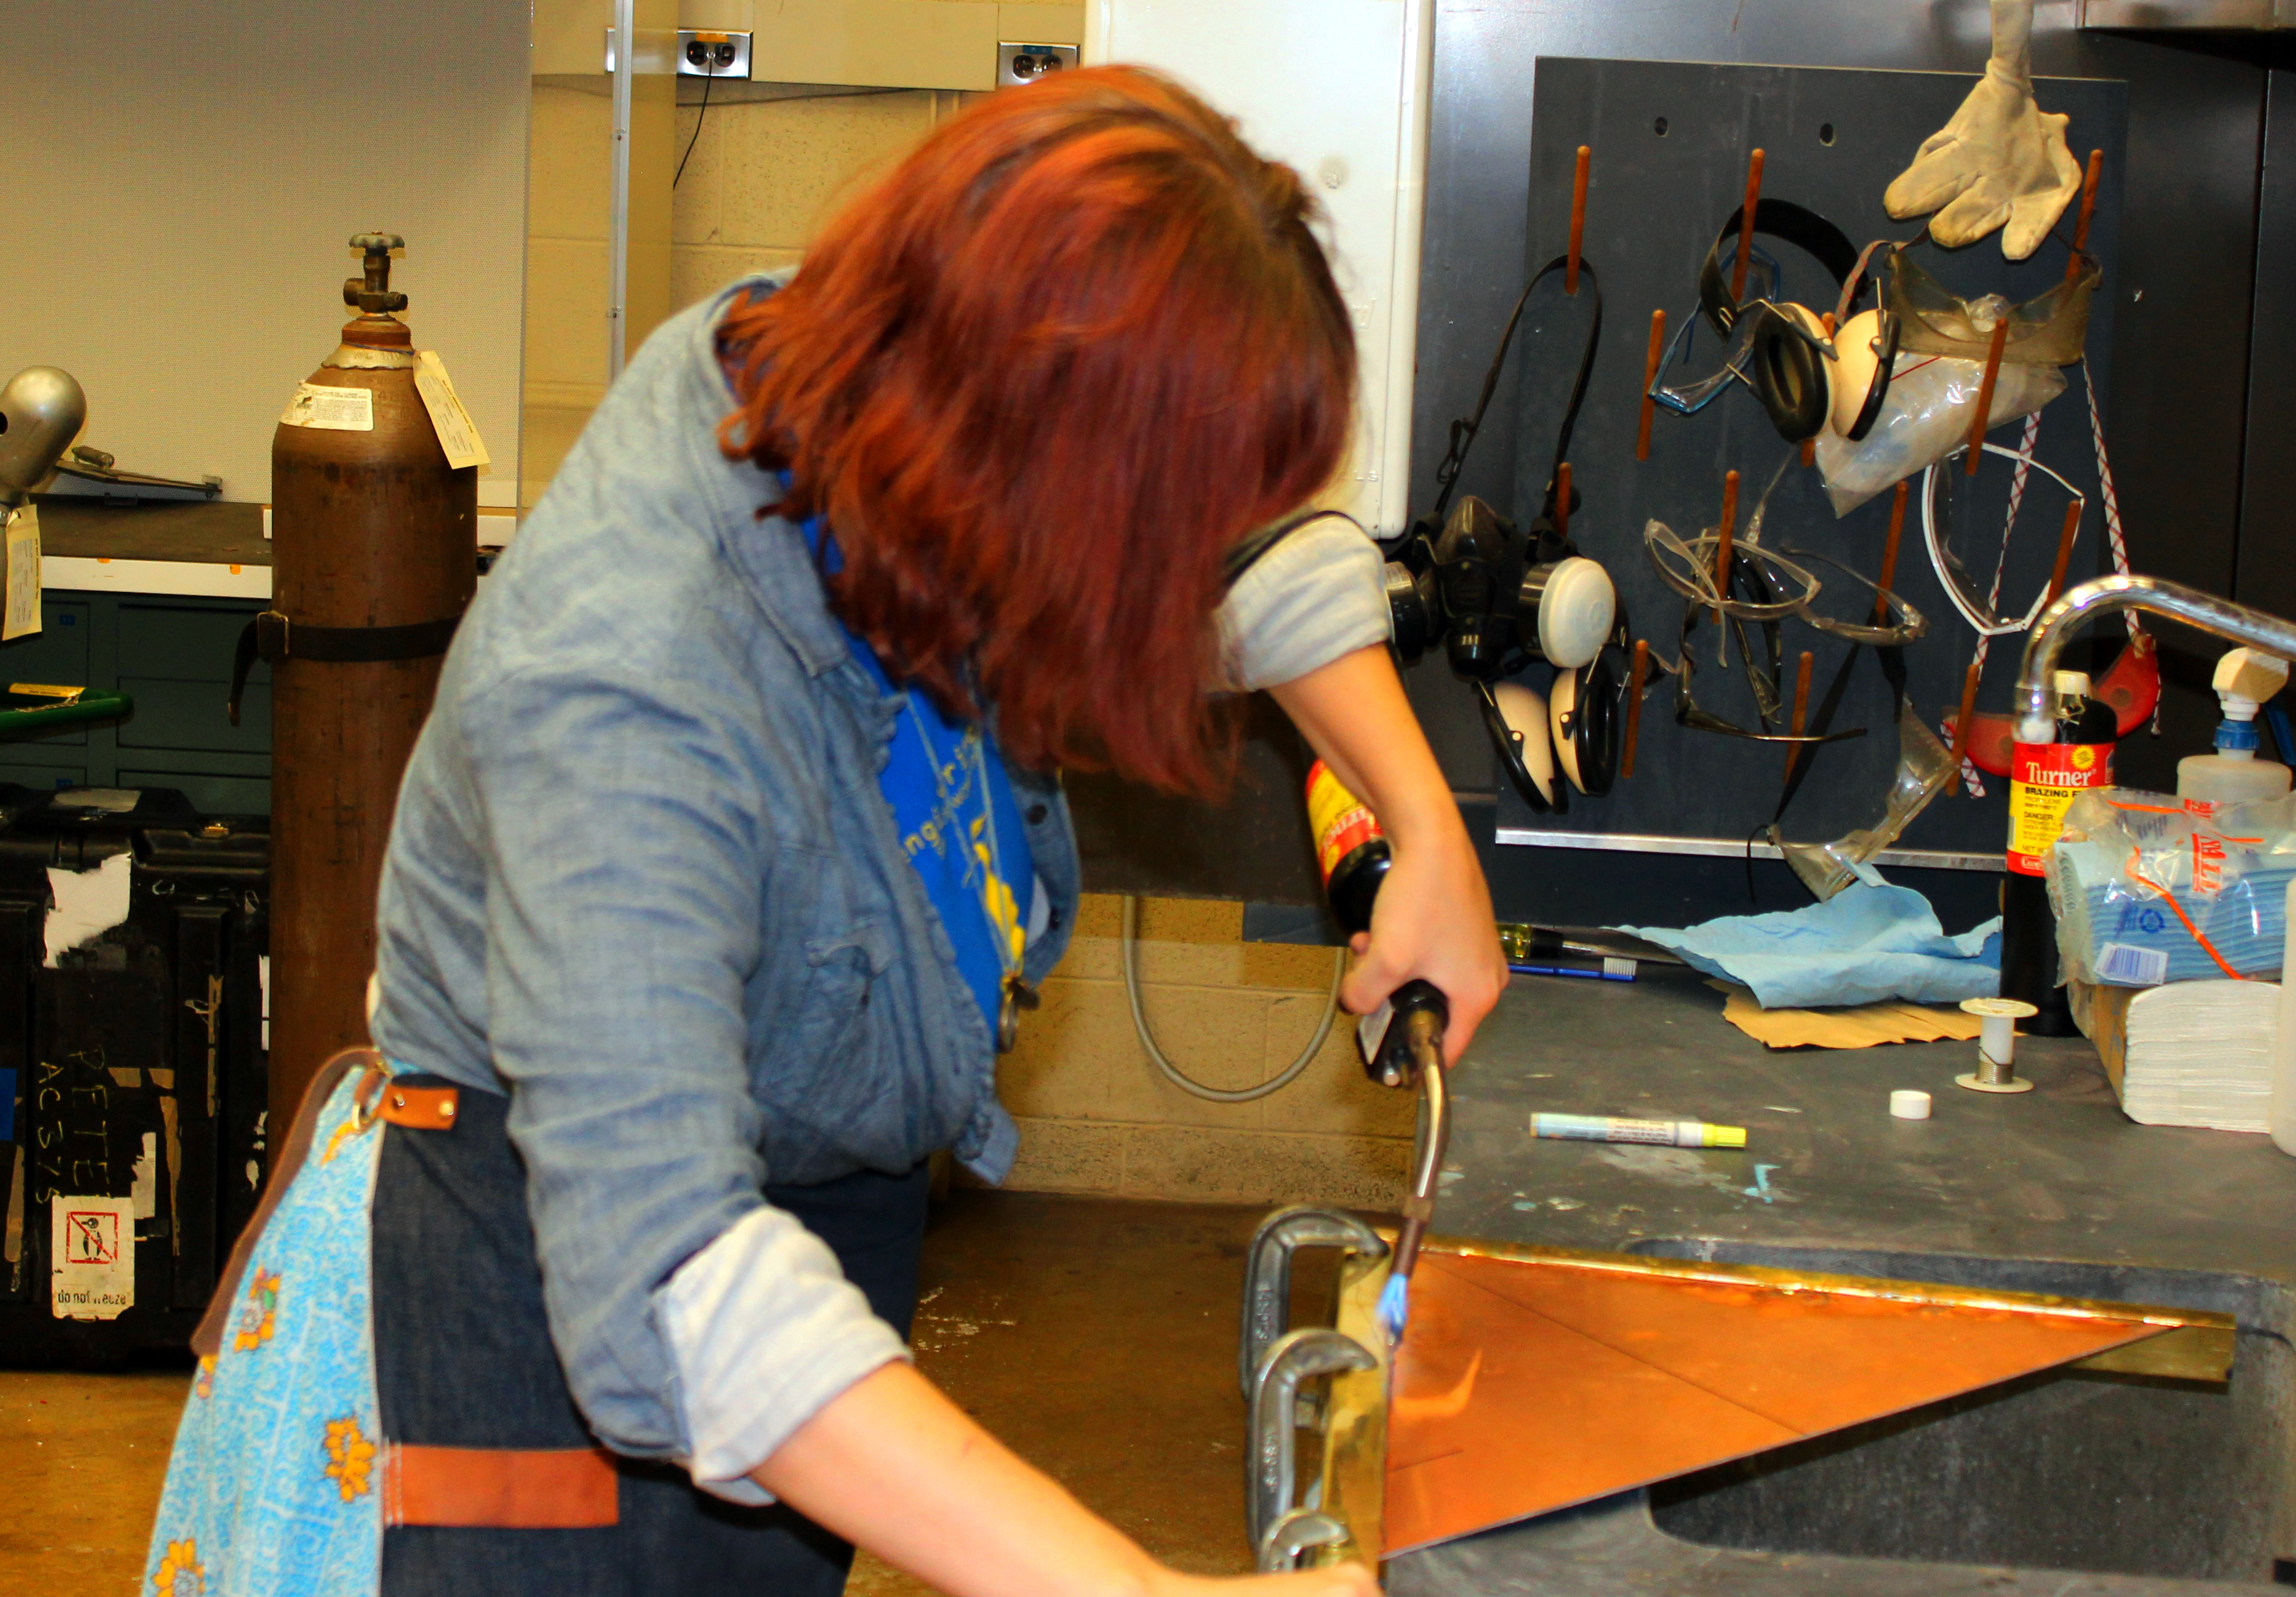
\includegraphics[width=0.95\linewidth]{SCIHI_system/figures/HIbiscus_solder.jpg}
\caption{Soldering the strip line to the HIbiscus antenna panels.}
\label{Fig:hibiscus_solder}
\end{minipage}
\end{figure} 

To construct the antenna petals, we started with large sheets of printed circuit board (pcb) material (see Figure \ref{Fig:hibiscus_pcb}). This material is a sheet of fiberglass sandwiched by two thin sheets of copper. We cut each of the trapezoidal shapes out of the pcb material, then added brass flanges to connect the shapes. Underneath the center line of each petal we placed a rib made out of aluminum angle with the appropriate bends to match the angles between trapezoids. Finally, the strip line panels were added using aluminum sheets soldered to some of the trapezoids (see Figure \ref{Fig:hibiscus_solder}). The entire system is bolted together using screws, and can be separated into parts for travel. 

\begin{figure}[htb]
\centering
\begin{minipage}[b]{0.52\textwidth}
\centering
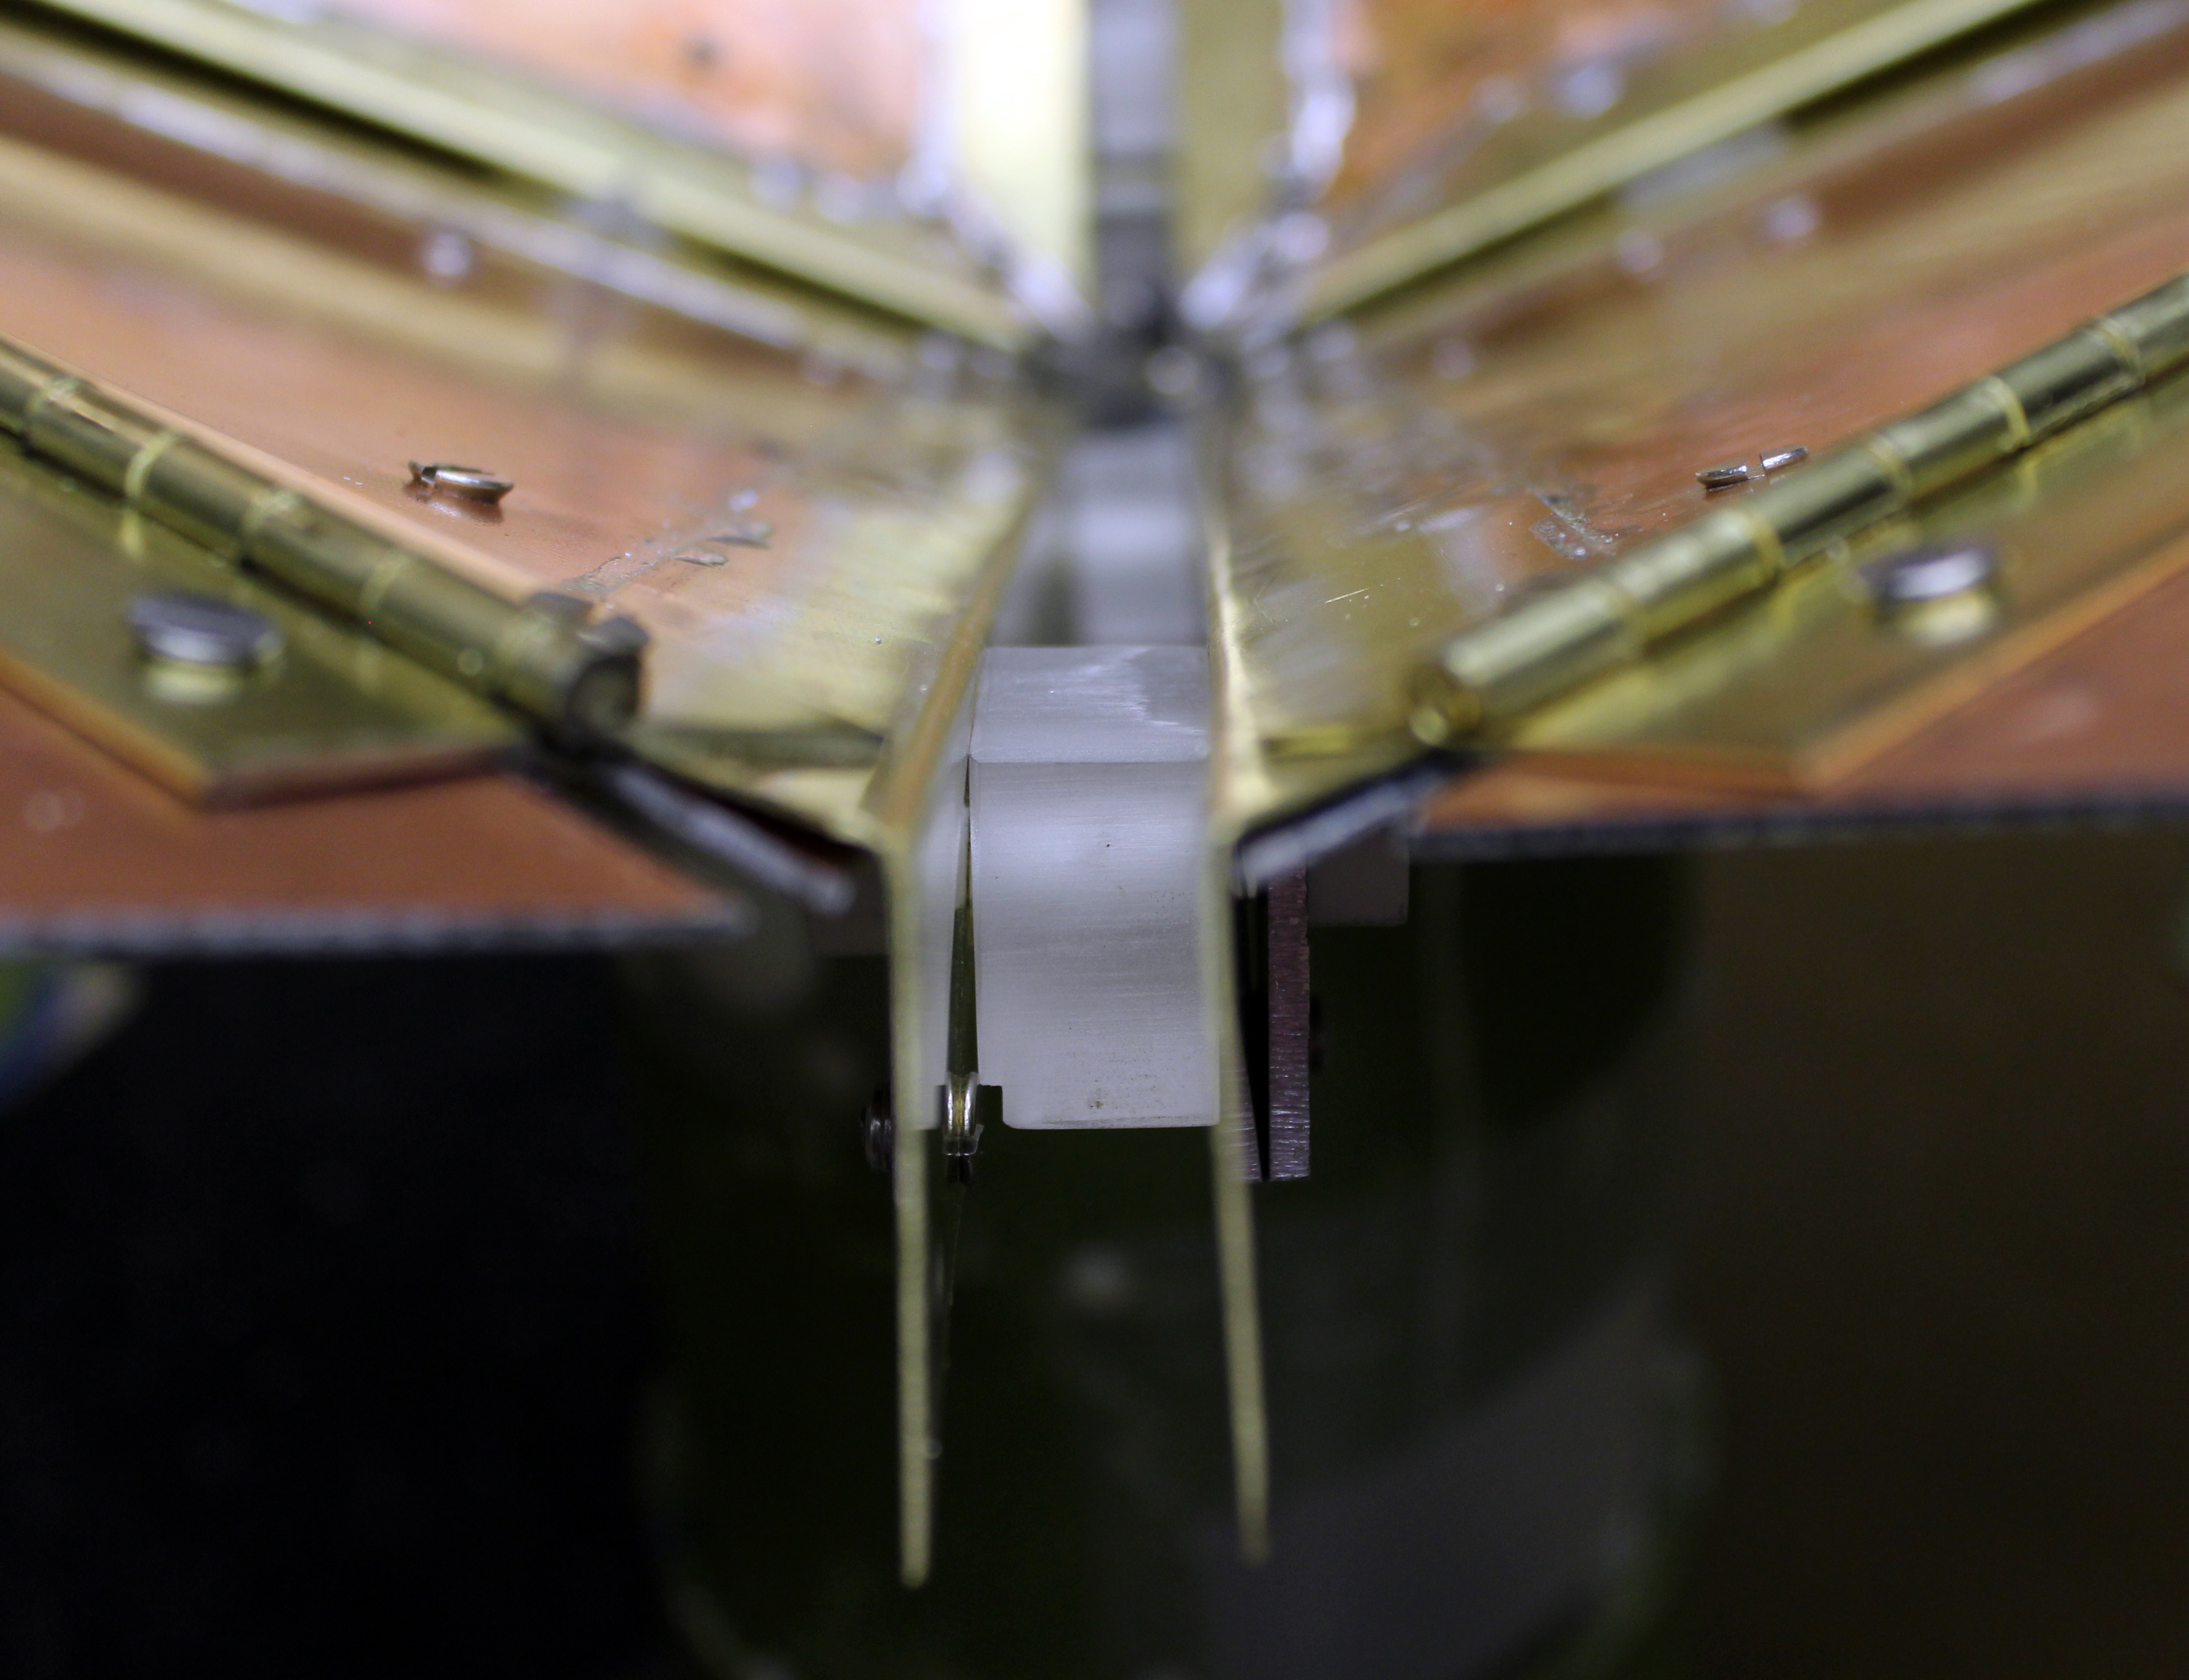
\includegraphics[width=0.95\linewidth]{SCIHI_system/figures/HIbiscus_strip_line.jpg}
\caption{Sight line down one of the strip lines for the HIbiscus antenna with spacers in place.}
\label{Fig:hibiscus_spacer}
\end{minipage}%
\begin{minipage}[b]{0.02\textwidth}
\hspace{1cm}
\end{minipage}%
\begin{minipage}[b]{0.42\textwidth}
\centering
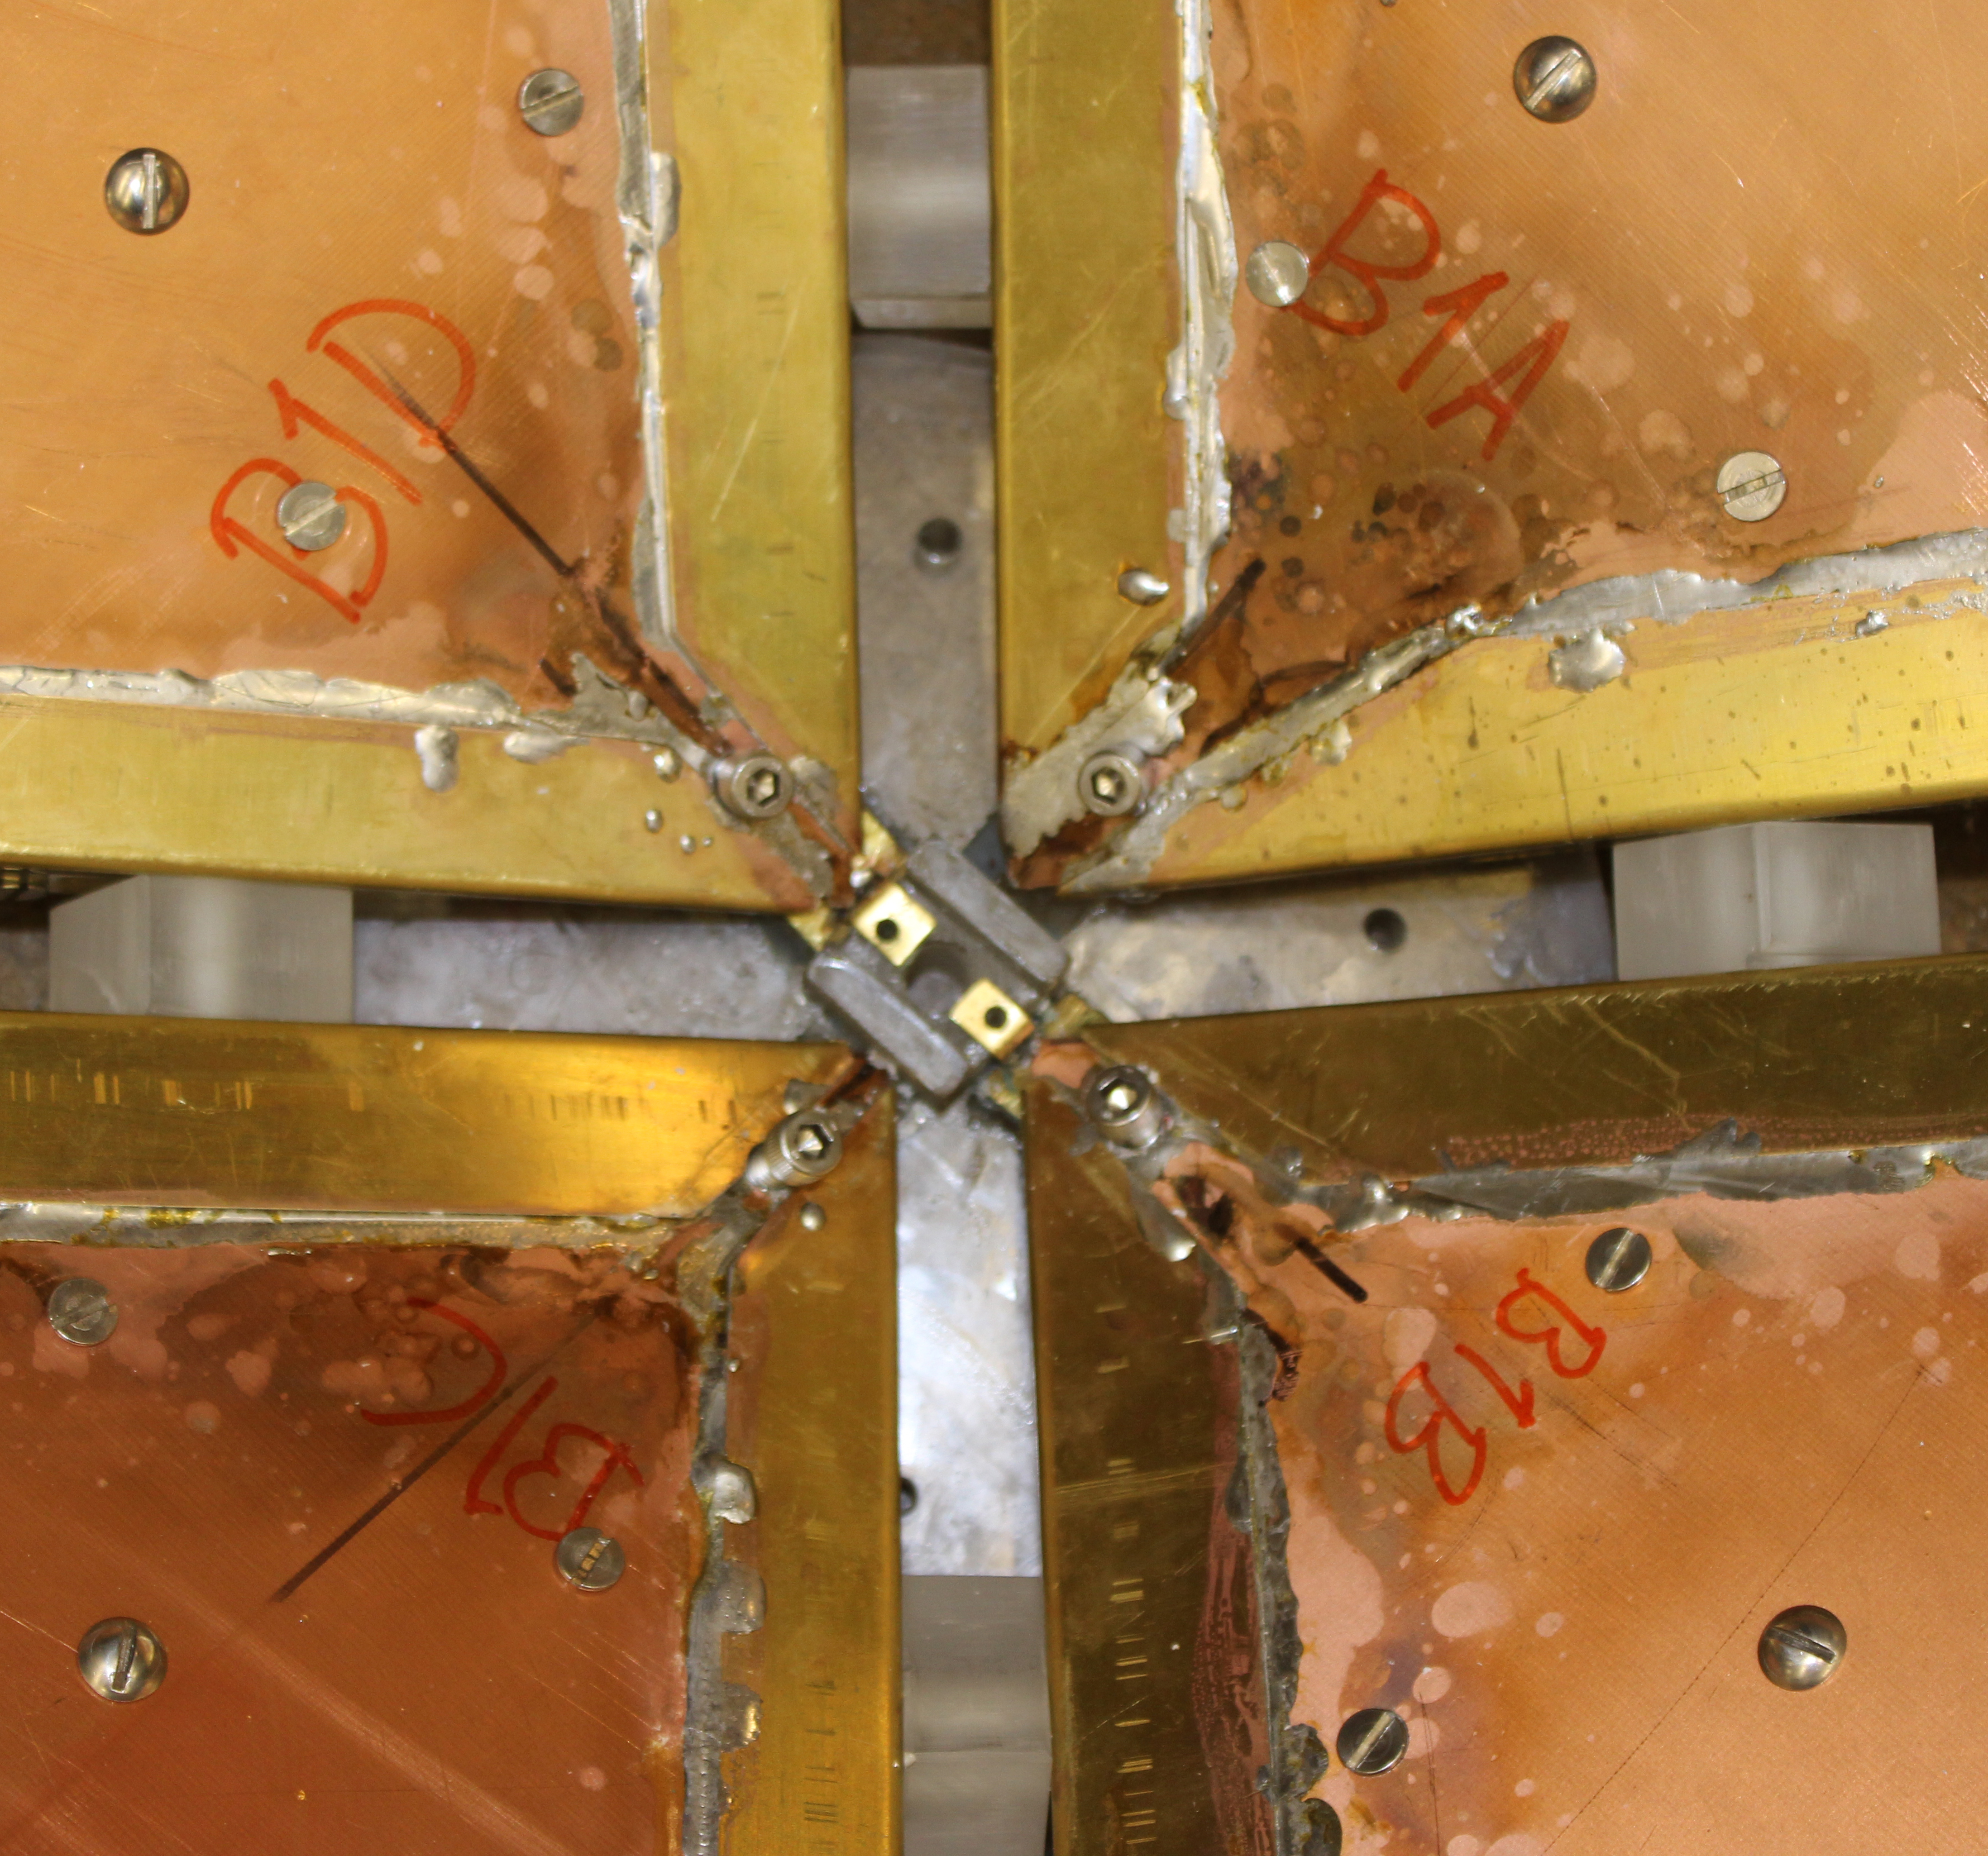
\includegraphics[width=0.95\linewidth]{SCIHI_system/figures/HIbiscus_center_point.jpg}
\caption{Center of the HIbiscus antenna with spacers and center mount block in place.}
\label{Fig:hibiscus_center}
\end{minipage}
\end{figure}

In order to keep the petal separation even and correct, lucite spacers were placed between each of the petals (see Figure \ref{Fig:hibiscus_spacer}). In addition, a lucite mount was built for the connection points at the center of the antenna (see Figure \ref{Fig:hibiscus_center}). The entire system was raised above the ground using a set of five PVC pipe legs; a central column and one leg for each petal (see Figure \ref{Fig:hibiscus_first}). 

With the antenna constructed, we could test that it matched our scale model measurements in terms of its s-parameters. To do this, we set up the antenna outdoors and made measurements with a portable Vector Network Analyzer. Measurements had to be made outdoors because the wavelengths corresponding to the SCI-HI frequencies ($40-130$ MHz) are $\sim$1-10 meters. This large wavelength scale means that reflections from the boundaries of a room can change antenna s-parameters, so accuracy in measurement requires the outdoor setting. Figures \ref{Fig:hibiscus_first} and \ref{Fig:hibiscus_gbt} show examples of how we made this measurement at CMU and Green Bank.

\textcolor{red}{Here I'll add a paragraph with S11 data using VNA and explanation.}

\subsubsection{Travelling with the Antenna}

\textcolor{red}{This section will describe how we packed up the original version of the HIbiscus antenna and travelled with it.}

\subsubsection{Antenna Upgrades}

\textcolor{red}{This section will describe the changes made to the HIbiscus antenna following last june's deployment including the new antennas that pack more neatly and have two different frequency ranges.}

\section{RF Electronics}

\subsection{Calibration Switch}

\subsection{Amplifiers}

\subsection{Impedence and Transmission Efficiency}

\subsection{Filters and Attenuation}

\section{Data Processing}

\subsection{Analog to Digital Conversion}

\subsection{Fourier Transformation and Data Collection Efficiency}

\subsection{Power Suppy and Consumption}

\subsection{Noise Generation and Shielding}

\subsubsection{Faraday Cage}

\subsubsection{Power Supply Noise}

